\chapter{Introduction}
\label{chapter:introduction}

%\emph{... \cite{example-article}}

\section{Background}
Over the years, many cities have gone through a transformation regarding surface and subsurface measures with the aim to mitigate and adapt to the consequences of climate change. Due to this transformation, the already heterogeneous and complex urban groundwater system faces an additional challenge regarding climate change. Two aspects that characterize the behavior of the urban groundwater system include surface sealing and systematic drainage of urban areas, resulting in surface runoff of precipitation to the sewage system next to replenishing the groundwater quantity through infiltration. (Ground)water nuisance can occur in urban areas, because the process of urbanisation does not include sustainable management of groundwater levels throughout the city \cite{ven-2007}.

City of Rotterdam manages an extensive groundwater monitoring network, consisting of approximately 2000 groundwater wells. The wells cover the entire municipal area of Rotterdam, reaching from urban to rural locations. The network is essential for addressing issues on for example foundations, subsidence, and (ground) water nuisance in basements throughout the municipal area, but is not intended to be used on a household level. Besides, monitoring groundwater data is crucial for understanding the groundwater dynamics within the municipality. The observed data by the municipality is used for civil technical measures and asset management. The construction of monitoring wells in public areas falls under municipal jurisdiction. Given its responsibility, it is essential not only to monitor groundwater levels but also to evaluate if the network density and well locations are efficient for optimal results \cite{geul-2022}.


\section{Problem statement}
Despite the distribution of the monitoring wells throughout the neighborhoods of Rotterdam, the uniformity of the monitoring wells also differs across them. One of the reasons is that City of Rotterdam only investigates the coverage of a subarea when a well is expired: They determine the necessity of well replacement and if the new well can be placed on a more optimal location. Consequently, the number of groundwater wells has been stagnant throughout the years and it is not know if the current number of monitoring wells is the most suitable number to retrieve groundwater information \cite{geul-2022}. Since groundwater is an integral part of the hydrological cycle, it is key to monitor and anticipate on the groundwater levels. Therefore, it is important to research the design of the network, analyze whether the network is optimal, and if monitoring wells need to be removed or reconstructed in a later stage \cite{european-environment-agency-2022}. An insufficient groundwater monitoring network could lead to consequences for urban planning, infrastructure, and environmental pollution. An insufficient network might form an obstacle regarding Rotterdam’s ability to mitigate and adapt to climate change impacts such as increased precipitation variability \cite{european-commission-2014}.

\newpage
\section{Research objective and questions}
Even though the number of monitoring wells has been stagnant over the past years, the network is currently an actively monitored groundwater network through the measurement of data loggers and manual collection. However, it is not known if the network is ideal yet. Therefore, the objective of the research study is to investigate the degree of optimization of the groundwater monitoring network of Rotterdam, see figure \labelcref{Research questions}. Incorporating the specified research questions into a methodology that blends theoretical insights with empirical investigations, the following research questions are outlined:

\begin{figure}[htbp]
    \centering
    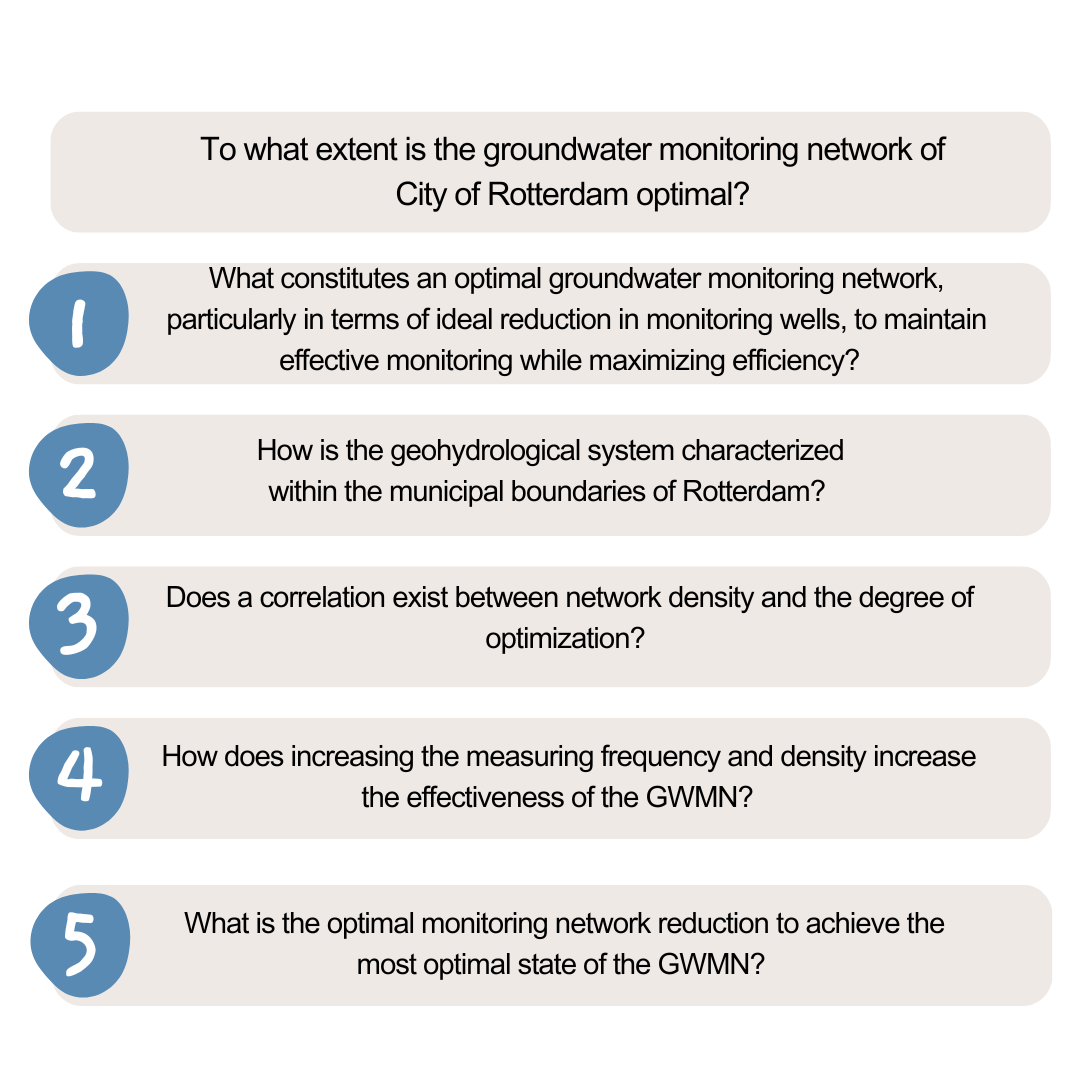
\includegraphics[width=0.75\linewidth]{figures/rq's-7.png}
    \caption{Main research question and five sub questions.}
    \label{Research questions}
\end{figure}
Summarizing, in the sub questions the following topics are researched and discussed: 
\begin{itemize}
    \item The definition of optimal in the context of a groundwater monitoring network;
    \item Characteristics of the geohydrological system of the municipal area of Rotterdam through visualization of geological information;
    \item The correlation between network density and the degree of optimization;
    \item Implications of optimizing the measuring frequency and coverage area of the monitoring wells;
    \item Comparison of reduction percentages to determine the optimal reduction rate to achieve an optimal state of the GWMN.

\end{itemize}

\newpage

\section{Social and scientific relevance}
The hypothesis driving this research suggests that the GWMN of Rotterdam has not reached its ideal state yet. This study is relevant as it explores the GWMN with a focus on an urban and industrial context. The primary goal is to evaluate the level of optimization of the GWMN through the development of a generic model using QR factorization. The findings of the research have the potential to serve as a valuable point of reference for other urban areas that face similar groundwater challenges. Accordingly, it is imperative to examine the GWMN to determine if sufficient and essential groundwater data are collected to make informed decisions for integrated groundwater management. A synergy between policy and execution is necessary to reach optimal groundwater management \cite{hoogvliet-2020}. The examination should include a critical examination on the spatial distribution and network density of the GWMN as well as the monitoring frequency. Ultimately, the research seeks to develop an approach for monitoring and optimizing Rotterdam's GWMN, offering contributions to societal and scientific fields. 

\section{Scope and delimitations}
The study focuses and explores on the following: 
\begin{itemize}
    \item The inclusion of active, phreatic monitoring wells; 
    \item The exclusion of project monitoring wells; 
    \item Case study areas Rozenburg and Heijplaat chosen from the municipal area of Rotterdam; 
    \item Project period of 2010-2024 with an optimization approach for 2020-2024; 
    \item Development of a generic model on neighborhood scale. 
\end{itemize}

\section{Reading guide}
The study begins with chapter \labelcref{chapter:Literature Review} "Literature Review", analyzing various methodologies to select the most suitable approach for this research. Followed by the chapter \labelcref{chapter:Theoretical Background} "Theoretical Background",  focusing on the hydrogeological context and management policies in The Netherlands. Chapter \labelcref{chapter:RM} discusses the approach, data collection and preparation, followed by two case studies of Rozenburg and Heijplaat. Chapter \labelcref{chapter:results} "Results", details results for both study areas. The study concludes with chapter \labelcref{chapter:discussion}, "Discussion", on the robustness of the model and reliability of the results, followed by chapter \labelcref{chapter:conclusion} "Conclusion" with aims to answer the research questions. The study ends with chapter \labelcref{chapter:recommendations} "Recommendations", highlighting the study limitations and suggesting directions for future research, aiming to enhance the understanding of Rotterdam's GWMN.













